\section{Il linguaggio della teoria degli insiemi}
Per non incorrere in contraddizione, accettiamo che le sole proposizioni ad avere senso siano quelle esprimibili mediante \vocab{formule insiemistiche}. Le formule si costruiscono ricorsivamente.
\begin{itemize}
	\item Le lettere $a,b,c,\ldots,A,B,C,\ldots,\alpha,\beta,\gamma,\ldots$ rappresentano \vocab{variabili}. I valori delle variabili sono sempre insiemi, e non ci sono altri oggetti salvo gli insiemi.
	\item Le \vocab{formule atomiche} sono:
	\[ \text{variabile = variabile} \qquad \qquad \text{variabile $\in$ variabile}\footnote{\,``appartiene a".}
		\]
	sono formule atomiche $x=y$, $x=x$, $\alpha = C$, e anche $x \in y$, $x \in x$, $\alpha \in C$.
	\item Le formule atomiche si combinano tra loro mediante:
	\begin{itemize}
		\item \vocab{connettivi logici} ovvero il ``non'' la ``e'' e la ``o'' (inclusiva):
		\[ \text{$\neg$ formula} \qquad \text{formula $\land$ formula} \qquad \text{formula $\lor$ formula}
			\]
		quindi ad esempio:
		\begin{flalign*}
			&\neg\Phi \equiv \text{``$\Phi$ è falsa''} &\\
			&\Phi \land \psi \equiv \text{``$\Phi$ e $\psi$ sono entrambe vere''} &\\
			&\Phi \lor \psi \equiv \text{``almeno una fra $\Phi$ e $\psi$ è vera''}
		\end{flalign*}
		\item \vocab{quantificatori} ovvero quello universale ``per ogni'' e quello esistenziale ``esiste'':
		\[ \forall x \, \text{formula} \qquad \exists x \, \text{formula}
			\]
		ad esempio:
		\begin{flalign*}
			&\forall x \, \Phi \equiv \text{``$\Phi$ è vera qualunque sia l'insieme $x$''} &\\
			&\exists x \, \Phi \equiv \text{``c'è un insieme $x$ che fa si che $\Phi$ sia vera''}
		\end{flalign*}
		\begin{exercise}
			Chiaramente varranno $\forall x \, x = x,$ $ \forall x \, \exists y \, x = y,$ $ \neg (\exists x \, \forall y \, x = y)$.
		\end{exercise}
	\end{itemize}
\end{itemize}

\textbf{\underline{L'intuizione}} è che l'universo insiemistico sia un gigantesco \href{https://it.wikipedia.org/wiki/Digrafo_aciclico}{\textcolor{purple}{grafo diretto aciclico}} i cui vertici sono gli insiemi,
ed in cui le frecce rappresentano la relazione di appartenenza.

\begin{center}
	\begin{figure}[h]
		\centering
		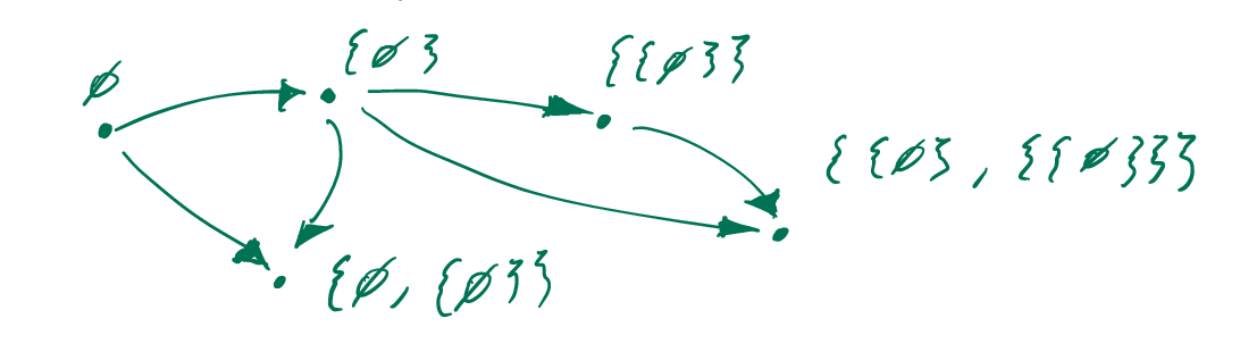
\includegraphics[width=10.5cm]{immagini/graf.png}
	\end{figure}
\end{center}

Possiamo solo fare affermazioni a proposito di vertici e frecce di questo grafo. Per esempio:
\[ \text{``$a$ è un elemento di un certo $b$''} \equiv \text{``c'è un percorso di due frecce fra $a$ e $b$''} 
	\]
che corrisponde mediante formule insiemistiche a $ \exists x (a \in x \land x \in b)$. E ancora:
\[\text{``$a$ è un sottoinsieme di $b$''} \equiv \text{``ogni elemento di $a$ è elemento di $b$''} \equiv \]\[
		\equiv\text{``non c'è un insieme che è elemento di $a$ e non di $b$''}\equiv\]\[
	 \equiv \text{``non c'è un vertice con una freccia verso $a$ e non una verso $b$''}
	\]
che corrisponde mediante formule insiemistiche a $\neg\exists x (x \in a \land \neg x \in b)$ (tutto ciò che raggiunge $a$ deve raggiungere anche $b$).\\
\textbf{\underline{Parentesi}} Ad essere precisi, avremmo dovuto definire le formule includendo un mucchio di parentesi, allo scopo di eliminare ogni possibilità
di formare una combinazione di simboli ambigua. Per esempio $\textcolor{red}{\Phi_1 \land \Phi_2 \lor \Phi_3}$ è ambigua, perché si potrebbe leggere $(\Phi_1 \land \Phi_2) \lor \Phi_3$
o $\Phi_1 \land (\Phi_2 \lor \Phi_3)$. In una notazione completamente parentesizzata, per esempio, la formula per ``$a$ è un sottoinsieme di $b$'' sarebbe:
\[ \neg(\exists x((x \in a)\land(\neg(x \in b))))
	\]
Non useremo, in generale, questa notazione, ma useremo le parentesi selettivamente per evitare ambiguità. \footnote{In questo caso si useranno più parentesi, qualora alcune formule risultassero più leggibili in tal modo.}\\
\textbf{\underline{Abbreviazioni}} Le formule appena descritte costituiscono il linguaggio della teoria degli insiemi \textbf{puro}. Durante il corso estenderemo
più volte questo linguaggio mediante abbreviazioni, che semplicemente rimpiazzano formule più lunghe con scritture convenzionali più compatte, e quindi non alterano 
la potenza espressiva del linguaggio. Vediamo le prime abbreviazioni:
\[ x \ne y \Mydef \neg x = y \footnote{Cioè ``non è vero che $x$ è uguale a $y$''.} \qquad x \not\in y \Mydef \neg x \in y \qquad \not\exists x \,\Phi \Mydef \neg \exists x \, \Phi
	\]\[ \Phi \rightarrow \psi \Mydef \psi \lor \neg \Phi \qquad \Phi \leftrightarrow \psi \Mydef (\Phi \rightarrow \psi) \land (\psi \rightarrow \Phi)
		\]\[ \exists x \in y \; \Phi \Mydef \exists x (x \in y \land \Phi) \qquad \forall x \in A \; \Phi \Mydef \forall x (x \in A \rightarrow \Phi)
			\]\[ \exists !\, x\, \Phi(x) \Mydef \exists x (\Phi(x) \land \forall y(\Phi(y) \rightarrow y = x))
				\]\[ \exists !\, x \in A \,\Phi(x) \Mydef \exists! \, x(x \in A \land \Phi(x))
					\]\[ A \subseteq B \Mydef \forall x (x \in A \rightarrow x \in B) \qquad A \subsetneq B \Mydef( A \subseteq B) \land (A \ne B)
						\]\[ C = A \cup B \Mydef \forall x \, x \in C \leftrightarrow (x \in A \lor x \in B)
							\]\[ C = A \cap B \Mydef \forall x \, x \in C \leftrightarrow (x \in A \land x \in B)
								\]
\begin{note}
	Il fatto che possiamo dire $C = A \cup B$ o $C = A \cap B$ non significa né che questi oggetti esistano né che siano unici. Dimostreremo fra poco l'esistenza e unicità 
	di unione e intersezione.
\end{note}

\begin{exercise}
Esprimi queste proposizioni mediante formule insiemistiche pure:
\begin{itemize}
	\item gli elementi degli elementi di $A$ sono elementi di $A$;
	\item $B$ è l'insieme dei sottoinsiemi di $A$;
	\item l'unione degli elementi di $A$ è l'intersezione di quelli di $B$\footnote{Qui assumi che l'unione e intersezione esistano e siano uniche.}
\end{itemize}
\end{exercise}

\subsection{Le regole di inferenza}
La teoria assiomatica degli insiemi si compone di tre parti: il linguaggio formale che abbiamo appena descritto, gli assiomi della teoria che studieremo durante il corso, 
ed un sistema di regole che specificano precisamente quali passaggi sono leciti nelle dimostrazioni. Possiamo immaginare questa ultima componente come una specie di algebra dei ragionamenti,
che permette di verificare i passaggi di una dimostrazione in maniera puramente meccanica, come se fossero semplici manipolazioni algebrica. Noi non vedremo le regole di inferenza, e voglio spiegare qui il perché.
\begin{enumerate}[1]
	\item Sono argomento del corso di logica.
	\item In realtà, scrivere le dimostrazioni in maniera formale, le renderebbe lunghissime e particolarmente incomprensibili.
	\item In pratica, non si sbaglia facendo ragionamenti che non reggono, si sbaglia dicendo cose fumose che non possono essere espresse nel linguaggio della teoria. Per esempio, le parole ``e così via'' sono pericolose.
	\item Conoscere le regole - fidatevi - non aiuta né a trovare né a capire le dimostrazioni.
\end{enumerate}
Pur senza dare un sistema completo di regole, vediamo qualche manipolazione formale che potrebbe servire.\\
\textbf{\underline{Tavole di verità}} Due combinazioni mediante connettivi logici ($\neg$, $\land$, $\lor$, $\rightarrow$, $\leftrightarrow$)
delle stesse formule - ``\vocab{combinazioni booleane}'' - alle volte, dicono la stessa cosa. Per esempio, $\neg \Phi \lor \neg \psi \equiv\footnote{\,``equivale a''.} \neg (\Phi \land \psi)$.
Per verificare questo fatto basta considerare tutte le possibili combinazioni di valori di verità che possono assumere le formule combinate - nell'esempio $\Phi$ e $\psi$ - compilando una ``\vocab{tabella di verità}''.
\begin{center}
	\begin{tabular}{>{$}l<{$}>{$}l<{$}|*{7}{>{$}l<{$}}}
	\Phi & \psi & \neg\Phi   & \neg\psi   & \neg\Phi \lor \neg\psi   & \Phi \land \psi & \neg(\Phi \land \psi)    \\
	\hline\vrule height 14pt width 0pt
	V & V & F & F & \textcolor{red}{F} & V & \textcolor{red}{F}\\
	V & F & F & V & \textcolor{red}{V} & F & \textcolor{red}{V}\\
	F & V & V & F & \textcolor{red}{V} & F & \textcolor{red}{V}\\
	F & F & V & V & \textcolor{red}{V} & F & \textcolor{red}{V}
	\end{tabular} 
\end{center}
Come si osserva le due colonne corrispondenti ai valori di verità delle nostre formule iniziali hanno gli stessi valori di verità in ogni caso.\\
Conviene tenere a mente alcune delle equivalenze elementari:
\[ \neg\neg \Phi \equiv \Phi \qquad \Phi \land (\psi \lor \Theta) \equiv (\Phi \land \psi) \lor (\Phi \land \Theta) \qquad \Phi \lor (\psi \land \Theta) \equiv (\Phi \lor \psi) \land (\Phi \lor \Theta)
	\]\[ \neg(\Phi \land \psi) \equiv \neg \Phi \lor \neg \psi \qquad \neg(\Phi \lor \psi) = \neg \Phi \land \neg \psi \, \footnote{\href{https://it.wikipedia.org/wiki/Leggi_di_De_Morgan}{\textcolor{purple}{Leggi di De Morgan}}.}
		\]\[ \Phi \rightarrow \neg \psi \equiv \psi \rightarrow \neg \Phi \qquad \Phi \rightarrow \psi \equiv \neg \psi \rightarrow \neg \Phi
			\]

\begin{exercise}
Dimostrare le equivalenze delle formule elencate sopra.
\end{exercise}

Per quanto riguarda i quantificatori ricordiamo le regole seguenti, che tuttavia non sono esaustive.
\[ \neg\forall x \, \Phi \equiv \exists x \, \neg\Phi \qquad \neg\forall x \, \neg \Phi \equiv \exists x \, \Phi
	\]\[ \neg\exists x \, \Phi \equiv \forall x \, \neg \Phi \qquad \neg \exists x \, \neg \Phi \equiv \forall x \, \Phi
		\]

\begin{exercise}
Convinciti della validità delle equivalenze precedenti.
\end{exercise}

\begin{exercise}
Dimostra che:
\[ \neg \forall x \in A \, \Phi \equiv \exists x \in A \, \neg \Phi \qquad \neg \exists x \in A \, \Phi \equiv \forall x \in A \, \Phi
	\]
\end{exercise}

\begin{exercise}
Dimostra che:
\[ \forall x (x \in A \rightarrow x \in B) \equiv \neg \exists x (x \in A \land \neg x \in B)
	\]
\end{exercise}

\begin{exercise}
Secondo te, la seguente formula è vera?
\[ \forall A ((\exists x \, x \in A) \rightarrow \exists x \in A (x \in B \rightarrow \forall y \in A \, y \in B))
	\]
\end{exercise}

Infine vi sono regole per la relazione di uguaglianza, che dicono, in sostanza, che se $x = y$ allora $x$ e $y$ non sono distinguibili, ossia vale $\Phi(x) \leftrightarrow \Phi(y)$ qualunque sia $\Phi$.
Per quanto ci riguarda, \textbf{se $x = y$ allora $x$ e $y$ sono nomi della stessa cosa}.